%=====================================================================
%  WARM NOTEBOOK -- cream background, sage/ochre/clay accents.
%  Signature motif: a segmented "fading" rule (long-to-short blocks
%  in a shifting color sequence) used under every title. Reusable
%  box and flowchart styles included, no literal plant/leaf imagery.
%=====================================================================
\documentclass[aspectratio=169,11pt]{beamer}
\usepackage[utf8]{inputenc}
\usepackage[T1]{fontenc}
\usepackage{helvet}
\renewcommand{\familydefault}{\sfdefault}
\usepackage{tikz}
\usetikzlibrary{arrows.meta,positioning,calc,shadows}
\tikzset{
  shadowy/.style={drop shadow={shadow xshift=1.6pt, shadow yshift=-1.8pt,
                               fill=ink, opacity=0.28}}
}

%---------------------------------------------------------------
% PALETTE
%---------------------------------------------------------------
\definecolor{paperbg}{HTML}{F3EFE4}   % warm cream background
\definecolor{ink}    {HTML}{2E2A22}   % warm near-black text
\definecolor{accent} {HTML}{5B7A57}   % sage green -- primary
\definecolor{accent2}{HTML}{B5793B}   % ochre -- secondary
\definecolor{accent3}{HTML}{A65A45}   % clay red -- tertiary
\definecolor{muted}  {HTML}{8A8371}   % warm grey, captions/footers
\definecolor{boxbg}  {HTML}{EAE4D4}   % slightly deeper cream, for boxes
\definecolor{boxline}{HTML}{C9BFA6}   % soft border tone

%---------------------------------------------------------------
% BASE BEAMER SETUP
%---------------------------------------------------------------
\usetheme{default}
\setbeamertemplate{navigation symbols}{}
\setbeamercolor{background canvas}{bg=paperbg}
\usebackgroundtemplate{\color{paperbg}\rule{\paperwidth}{\paperheight}}
\setbeamercolor{normal text}{fg=ink}
\setbeamercolor{structure}{fg=accent}
\setbeamercolor{itemize item}{fg=accent}
\setbeamerfont{frametitle}{size=\Large,series=\bfseries}
\setbeamercolor{frametitle}{fg=ink}
\setbeamertemplate{itemize items}[circle]

%---------------------------------------------------------------
% SIGNATURE MOTIF: segmented fading rule
%---------------------------------------------------------------
\newcommand{\fadebar}[2][1.4pt]{%
  \begin{tikzpicture}[baseline=-0.5ex, x=1cm, y=1cm]
    \pgfmathsetmacro{\wa}{#2*0.46}
    \pgfmathsetmacro{\wb}{#2*0.28}
    \pgfmathsetmacro{\wc}{#2*0.16}
    \pgfmathsetmacro{\wd}{#2*0.10}
    \useasboundingbox (0,0) rectangle (#2,#1);
    \fill[accent]  (0,0) rectangle (\wa,#1);
    \pgfmathsetmacro{\bstart}{\wa+0.03}
    \pgfmathsetmacro{\bend}{\bstart+\wb}
    \fill[accent2] (\bstart,0) rectangle (\bend,#1);
    \pgfmathsetmacro{\cstart}{\bend+0.03}
    \pgfmathsetmacro{\cend}{\cstart+\wc}
    \fill[accent3] (\cstart,0) rectangle (\cend,#1);
    \pgfmathsetmacro{\dstart}{\cend+0.03}
    \pgfmathsetmacro{\dend}{\dstart+\wd}
    \fill[muted]   (\dstart,0) rectangle (\dend,#1);
  \end{tikzpicture}%
}

% -- Compact frametitle to reclaim vertical space on every slide --
\setbeamertemplate{frametitle}{
  \vspace*{0.15cm}
  \hspace*{0.9cm}\usebeamerfont{frametitle}\insertframetitle\par
  \vspace{3pt}
  \hspace*{0.9cm}\fadebar{2.6}
  \vspace{0.1cm}
}
\setbeamertemplate{footline}{
  \hfill\textcolor{muted}{\tiny\insertframenumber\,/\,\inserttotalframenumber}\hspace*{0.6cm}\vspace{0.3cm}
}
\setbeamersize{text margin left=0.9cm,text margin right=0.9cm}

%---------------------------------------------------------------
% REUSABLE BOX STYLES
%---------------------------------------------------------------
\newenvironment{notebox}[1][]{%
  \begin{tcolorbox}[
      enhanced, breakable,
      colback=boxbg, colframe=boxline,
      boxrule=0.5pt, arc=1pt,
      left=8pt, right=8pt, top=4pt, bottom=4pt,
      title={#1},
      colbacktitle=boxbg, coltitle=ink,
      fonttitle=\bfseries\small,
      titlerule=0pt,
      drop shadow,
      borderline north={1.6pt}{0pt}{accent},
      overlay unbroken and first={
        \draw[accent2, line width=0.9pt]
          ([xshift=0pt]frame.north west) -- ++(0,-0.28);
      }
    ]
}{\end{tcolorbox}}

\newcommand{\flag}[2][accent]{%
  \tikz[baseline=-0.5ex]{
    \node[fill=#1, text=paperbg, font=\bfseries\scriptsize,
          inner sep=3pt, rounded corners=1pt, minimum width=6pt, shadowy] {#2};
  }%
}

%---------------------------------------------------------------
% FLOWCHART STYLE
%---------------------------------------------------------------
\tikzset{
  flownode/.style={
    rectangle, rounded corners=3pt,
    draw=boxline, line width=0.8pt, fill=boxbg,
    text=ink, font=\small\bfseries, align=center,
    minimum height=0.95cm, inner sep=7pt, shadowy
  },
  flownodealt/.style={
    flownode, draw=accent3, fill=accent3!12
  },
  flowarrow/.style={
    -{Latex[length=2.2mm, width=1.6mm]}, line width=0.9pt, draw=accent
  },
  flowlabel/.style={font=\tiny, text=muted}
}
\usetikzlibrary{shadows}

\title{2D Positional-Audio Sandbox}
\author{Team ABC -- CSE 220}
\institute{Dept. of CSE, BUET}
\date{\\Sabir Siam : 2305061\\ Anindya Nag Arghya : 2305086}

\usepackage{tcolorbox}
\tcbuselibrary{skins,breakable}

\begin{document}

\setlength{\abovedisplayskip}{3pt}
\setlength{\belowdisplayskip}{3pt}
\setlength{\abovedisplayshortskip}{1pt}
\setlength{\belowdisplayshortskip}{1pt}

%=====================================================================
% FRAME 1 -- TITLE
%=====================================================================
\begin{frame}[plain]
  \vspace{1.7cm}
  \flag[accent2]{FINAL PROJECT}\;\textcolor{muted}{\small \insertinstitute}\par
  \vspace{0.35cm}
  {\Huge\bfseries \inserttitle}\par
  \vspace{0.4cm}
  \fadebar{3.4}\par
  \vspace{0.5cm}
  {\large \insertauthor}\par
  {\small\textcolor{muted}{\insertdate}}
\end{frame}

%=====================================================================
% FRAME 2 -- PROJECT AT A GLANCE
%=====================================================================
\begin{frame}{Project at a Glance}
  \begin{columns}[T]
    \begin{column}{0.50\textwidth}
      \small
      A real-time \textbf{2D positional-audio engine}. Place a listener
      and sources on a grid, paint walls, and hear -- live -- how
      distance, obstruction, material, and reflection change the sound:
      \begin{itemize}\itemsep2.5pt
        \item \textcolor{accent3}{\textbf{Muffling}} as paths get obstructed
        \item \textbf{Panning} as sources move left / right
        \item Delayed, directional \textbf{echoes}
        \item Sound \textbf{bleeding through} walls
      \end{itemize}

      \vspace{14pt}
      \flag[accent]{PYTHON}\;\flag[accent2]{PYGAME}\;\flag[accent3]{NUMPY}\;\flag[muted]{SOUNDDEVICE}
    \end{column}
    \begin{column}{0.46\textwidth}
      \centering
      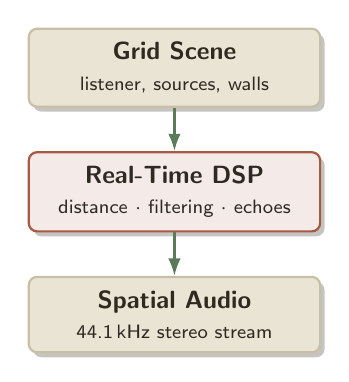
\begin{tikzpicture}[
          node distance=0.55cm,
          gnode/.style={flownode, minimum width=3.7cm, minimum height=0.82cm, inner sep=5pt, font=\small\bfseries},
          gnodealt/.style={flownodealt, minimum width=3.7cm, minimum height=0.82cm, inner sep=5pt, font=\small\bfseries}
        ]
        \node[gnode] (a) {Grid Scene\\\scriptsize\normalfont listener, sources, walls};
        \node[gnodealt, below=of a] (b) {Real-Time DSP\\\scriptsize\normalfont distance $\cdot$ filtering $\cdot$ echoes};
        \node[gnode, below=of b] (c) {Spatial Audio\\\scriptsize\normalfont 44.1\,kHz stereo stream};
        \draw[flowarrow] (a) -- (b);
        \draw[flowarrow] (b) -- (c);
      \end{tikzpicture}\par
      \vspace{6pt}
      {\scriptsize\textcolor{muted}{\textit{Live, interactive $\cdot$ all in Python}}}
    \end{column}
  \end{columns}
\end{frame}

%=====================================================================
% FRAME -- MOTIVATION / COLD OPEN
%=====================================================================
\begin{frame}{Motivation: Beyond Empty Space}
  \begin{columns}[T]
    \begin{column}{0.50\textwidth}
      \small
      \textbf{\textcolor{accent}{Free Space is Trivial}}
      \begin{itemize}\itemsep1pt
        \item Moving away $\to$ volume drops ($\text{gain}\propto 1/d$)
        \item Moving sideways $\to$ stereo pan (left / right)
      \end{itemize}
      \vspace{2pt}
      {\scriptsize\textcolor{muted}{In a void, spatial audio is just basic amplitude scaling.}}

      \vspace{8pt}
      \textbf{\textcolor{accent3}{Real Rooms Have Geometry}}
      \begin{itemize}\itemsep1pt
        \item \textbf{Corners \& edges} -- diffract and muffle highs
        \item \textbf{Solid walls} -- absorb, let muffled sound bleed through
        \item \textbf{Surfaces} -- generate delayed, directional echoes
      \end{itemize}
    \end{column}
    \begin{column}{0.46\textwidth}
      \begin{notebox}[The Central Challenge]
        \small\textit{``Can we simulate walls, materials, and echoes
        convincingly, live, using \textbf{only} the signal-processing
        tools this course taught us?''}

        \vspace{4pt}
        \flag[accent]{IN SCOPE}\; {\scriptsize Fourier, DFT, FFT, convolution}\\[3pt]
        \flag[accent3]{OUT OF SCOPE}\; {\scriptsize Laplace/Z-transforms, IIR cascades}

        \vspace{4pt}
        {\scriptsize\textcolor{muted}{Goal: a real-time (44.1\,kHz)
        interactive sandbox, built from FFT multiplication,
        delay lines, and 2D grid search.}}
      \end{notebox}
    \end{column}
  \end{columns}
\end{frame}

%=====================================================================
% FRAME A -- THREE INPUT MODES
%=====================================================================
\begin{frame}{Audio Input Pipeline: Three Operational Modes}
  \begin{columns}[T]
    \begin{column}{0.315\textwidth}
      \begin{notebox}[]
        \flag[accent]{MODE 1: AUDIO FILE}\par
        \vspace{6pt}
        \raggedright\scriptsize
        \textbf{Format:}\; \texttt{.wav}, \texttt{.flac}, \texttt{.mp3}\\[3pt]
        \textbf{Pipeline:}\; Eagerly loaded into \texttt{float32} NumPy memory\\[3pt]
        \textbf{Role:}\; Instant testing with no audio hardware needed
      \end{notebox}
    \end{column}
    \begin{column}{0.315\textwidth}
      \begin{notebox}[]
        \flag[accent2]{MODE 2: LOCAL MIC}\par
        \vspace{6pt}
        \raggedright\scriptsize
        \textbf{Format:}\; Live microphone hardware\\[3pt]
        \textbf{Pipeline:}\; \texttt{sounddevice} circular stream buffer\\[3pt]
        \textbf{Role:}\; Real-time voice testing directly in the room
      \end{notebox}
    \end{column}
    \begin{column}{0.315\textwidth}
      \begin{notebox}[]
        \flag[accent3]{MODE 3: NETWORK UDP}\par
        \vspace{6pt}
        \raggedright\scriptsize
        \textbf{Format:}\; Remote Wi-Fi/Ethernet clients\\[3pt]
        \textbf{Pipeline:}\; UDP port \texttt{50007} to thread-safe queues\\[3pt]
        \textbf{Role:}\; Multi-source relay with client auto-reclaim
      \end{notebox}
    \end{column}
  \end{columns}

  \vspace{10pt}
  \begin{notebox}[]
    \centering\footnotesize
    \flag[accent]{HARDWARE VERIFIED}\quad
    \textcolor{ink}{\textbf{Live Multi-Device Validation:}}
    \textcolor{muted}{Mode 3 verified across physical laptops on an active LAN, firewall traversal included.}
  \end{notebox}
\end{frame}

%=====================================================================
% FRAME B -- NETWORKED STREAMING & SAMPLING PARAMETERS
%=====================================================================
\begin{frame}{Networked Streaming \& Sampling Parameters}
  \begin{columns}[T]
    \begin{column}{0.48\textwidth}
      \small\textbf{\textcolor{accent}{Network Plumbing}} {\scriptsize(\texttt{network\_input.py})}
      \begin{itemize}\itemsep1pt
        \item \textbf{Transport:} UDP port \texttt{50007} -- drops packets over buffer stalls
        \item \textbf{Packet format:} 32-bit float PCM, 1024 samples per datagram
        \item \textbf{Lifecycle:} background listener $\to$ queues; idle timeout $\approx\!5$\,s
      \end{itemize}
    \end{column}
    \begin{column}{0.48\textwidth}
      \small\textbf{\textcolor{accent3}{Sampling \& Latency Budget}}
      \begin{itemize}\itemsep1pt
        \item \textbf{Nyquist--Shannon:} $f_{\max}\!\approx\!20$\,kHz $\Rightarrow f_s = 44.1$\,kHz (no aliasing)
        \item \textbf{Block size $N\!=\!1024$:}\; $\Delta t = N/f_s \approx 23.2$\,ms per buffer
        \item Short enough to feel instant, long enough for stable FFTs
      \end{itemize}
    \end{column}
  \end{columns}

  \vspace{10pt}
  \centering
  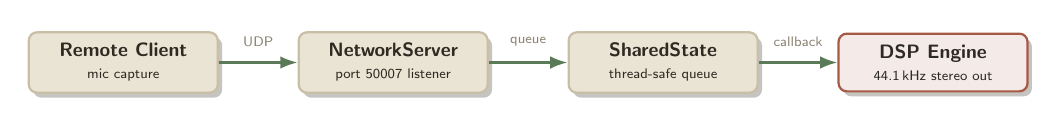
\begin{tikzpicture}[
      node distance=1.0cm,
      hnode/.style={flownode, minimum width=2.4cm, minimum height=0.65cm, inner sep=4pt, font=\scriptsize\bfseries},
      hnodealt/.style={flownodealt, minimum width=2.4cm, minimum height=0.65cm, inner sep=4pt, font=\scriptsize\bfseries}
    ]
    \node[hnode] (a) {Remote Client\\\tiny\normalfont mic capture};
    \node[hnode, right=of a] (b) {NetworkServer\\\tiny\normalfont port 50007 listener};
    \node[hnode, right=of b] (c) {SharedState\\\tiny\normalfont thread-safe queue};
    \node[hnodealt, right=of c] (d) {DSP Engine\\\tiny\normalfont 44.1\,kHz stereo out};

    \draw[flowarrow] (a) -- (b) node[midway, above=2pt, flowlabel]{UDP};
    \draw[flowarrow] (b) -- (c) node[midway, above=2pt, flowlabel]{queue};
    \draw[flowarrow] (c) -- (d) node[midway, above=2pt, flowlabel]{callback};
  \end{tikzpicture}
\end{frame}

%=====================================================================
% FRAME -- CHALLENGE 1: PROBLEM STATEMENT
%=====================================================================
\begin{frame}{Challenge 1: The Intuitive Starting Point}
  \vspace{8pt}
  {\large\textit{``Let's start with the absolute basics: if a sound
  source is farther away, it should sound quieter. If it moves to
  your left, you should hear it in your left ear.''}}

  \vspace{14pt}
  \centering
  \begin{notebox}[]
    \centering
    \flag[accent]{THE CHALLENGE}

    \vspace{4pt}
    \normalsize How do we translate simple 2D grid coordinates
    $(x, y)$ into natural volume attenuation and stereo balance ---
    without complex 3D physics?
  \end{notebox}

  \vspace{12pt}
  \raggedright
  \begin{itemize}
    \item \textbf{Distance:} amplitude must decay smoothly -- no sudden dropoffs, no infinite volume at zero range
    \item \textbf{Direction:} horizontal displacement must pan smoothly without losing volume when centered
  \end{itemize}

  \vspace{10pt}
  \textcolor{muted}{\scriptsize $\implies$ Next: translating spatial geometry into basic signal scaling and linear panning.}
\end{frame}

%=====================================================================
% FRAME -- CHALLENGE 1 SOLUTION (A): DISTANCE & DIRECTION FORMULAS
%=====================================================================
\begin{frame}{Challenge 1: Distance \& Direction --- Formulas}
  \begin{columns}[T]
    \begin{column}{0.48\textwidth}
      \flag{INVERSE-DISTANCE}
      \vspace{3pt}
      \small\textbf{Distance attenuation}
      \[
        g(d) = \frac{1.0}{1.0 + k \cdot d}
      \]
      {\scriptsize\textcolor{muted}{$k = 0.08$ -- tuned by ear on a $40\times24$ grid.}}

      \vspace{6pt}
      \flag[accent2]{STEREO PAN}
      \vspace{3pt}
      \small\textbf{Linear azimuthal panning}
      \[
        \text{pan} = \text{clip}\!\left(\frac{\Delta x}{20.0},\, -1,\, 1\right),\quad
        \Delta x = x_{\text{src}} - x_{\text{lis}}
      \]
      \[
        g_L = \tfrac{1-\text{pan}}{2}, \qquad
        g_R = \tfrac{1+\text{pan}}{2}
      \]
    \end{column}
    \begin{column}{0.48\textwidth}
      \flag[accent3]{COMBINED STEREO OUTPUT}
      \vspace{3pt}
      \small\textbf{Per-sample signal vector}
      \[
        \mathbf{y}[n] = \begin{bmatrix} g_L\, g(d)\, x[n] \\ g_R\, g(d)\, x[n] \end{bmatrix}
      \]

      \vspace{6pt}
      \begin{notebox}[Key Properties]
        \scriptsize
        \begin{itemize}\itemsep1pt
          \item Constant total gain: $g_L + g_R = 1$ -- no volume dip at center
          \item Smooth decay: no singularity at $d{=}0$
          \item Pure NumPy: \texttt{mono * gain * pan}
        \end{itemize}
      \end{notebox}
    \end{column}
  \end{columns}
\end{frame}

%=====================================================================
% FRAME -- CHALLENGE 1 SOLUTION (B): SYLLABUS TIE-IN & DEMO
%=====================================================================
\begin{frame}{Challenge 1: Signal Scaling in Practice}
  \begin{columns}[T]
    \begin{column}{0.48\textwidth}
      \flag[accent]{SYLLABUS TIE-IN: SCALAR MULTIPLICATION}
      \vspace{3pt}
      \small
      \textbf{The fundamental operation:}\; $y[n] = A \cdot x[n]$
      \begin{itemize}\itemsep2pt
        \item Time-domain scalar multiplication -- the simplest linear transform
        \item Spatial audio starts as amplitude modulation across two channels
        \item This is the \textit{baseline} before any frequency-domain or delay-based effects
      \end{itemize}
    \end{column}
    \begin{column}{0.48\textwidth}
      \flag[accent2]{IMPLEMENTATION}
      \vspace{3pt}
      \small
      \begin{notebox}[Implementation Details]
        \scriptsize Pure NumPy vectorization: \texttt{mono * gain * pan}.
        No per-sample Python loops -- entire 1024-sample block
        processed in one NumPy broadcast.
      \end{notebox}
      \vspace{6pt}
      \begin{notebox}[Live Demo Cue]
        \flag[accent2]{DEMO CUT}\; \scriptsize Move a single source
        circularly around the stationary listener on an open grid --
        volume and stereo balance shift live.
      \end{notebox}
    \end{column}
  \end{columns}
\end{frame}

%=====================================================================
% FRAME -- CHALLENGE 2: PROBLEM STATEMENT
%=====================================================================
\begin{frame}{Challenge 2: Obstacles \& Acoustic Character}
  \vspace{8pt}
  {\large\textit{``A wall shouldn't just be an ON/OFF mute switch. In
  real life, when someone speaks behind a door, you still hear them
  --- it just sounds duller, muffled, like the treble was stripped
  away.''}}

  \vspace{14pt}
  \centering
  \begin{notebox}[]
    \centering
    \flag[accent]{THE CHALLENGE}

    \vspace{4pt}
    \normalsize How do we simulate acoustic ``muffling'' dynamically
    in real time --- changing the spectral character of the signal,
    rather than just cutting its volume?
  \end{notebox}

  \vspace{12pt}
  \raggedright
  \begin{itemize}
    \item Sound doesn't just stop; high frequencies are absorbed far faster than low frequencies
    \item We need a lowpass filter whose cutoff adapts dynamically to obstacles
  \end{itemize}

  \vspace{10pt}
  \textcolor{muted}{\scriptsize $\implies$ Next: the obvious textbook solution, and why our syllabus forced us to build something better.}
\end{frame}

%=====================================================================
% FRAME -- FILTERING: THE SYLLABUS DILEMMA (IIR VS. FFT)
%=====================================================================
\begin{frame}{Filtering: The Syllabus Dilemma (IIR vs.\ FFT)}
  \begin{columns}[T]
    \begin{column}{0.48\textwidth}
      \flag[accent3]{REJECTED: BUTTERWORTH IIR}
      \vspace{3pt}
      \small
      \begin{itemize}\itemsep2pt
        \item Standard approach: 2nd-order Butterworth lowpass via \texttt{scipy.signal.sosfilt}
        \item \textbf{Problem:} Butterworth design requires the \textbf{Z-transform} (bilinear transform, pole stability)
        \item Z-transforms are taught \textbf{weeks later} -- defending IIR before covering the theory was a non-starter
      \end{itemize}
    \end{column}
    \begin{column}{0.48\textwidth}
      \flag[accent]{ADOPTED: PER-BLOCK FFT FILTER}
      \vspace{3pt}
      \small
      \begin{itemize}\itemsep2pt
        \item What the syllabus \textit{did} teach: DFT, FFT, frequency-domain multiplication
        \item \textbf{Decision:} build a custom frequency-domain filter from scratch with \texttt{rfft}/\texttt{irfft}
      \end{itemize}
      \vspace{4pt}
      \begin{notebox}[The Academic Philosophy]
        \scriptsize\textit{Better to implement a first-principles FFT
        filter we can rigorously defend than drop in an
        unexplained IIR library.}
      \end{notebox}
    \end{column}
  \end{columns}
\end{frame}

%=====================================================================
% FRAME -- FFT LOWPASS (A): THE RAISED-COSINE FILTER
%=====================================================================
\begin{frame}{Per-Block FFT Lowpass: The Raised-Cosine Filter}
  \begin{columns}[T]
    \begin{column}{0.5\textwidth}
      \flag{PER-BLOCK FFT}\;\flag[accent2]{RAISED-COSINE}
      \vspace{3pt}
      \small
      Transform to frequency domain:
      \[
        X[k] = \text{rfft}(x[n]), \quad k = 0,\dots,N/2
      \]
      Raised-cosine gain curve $H(f)$, 500\,Hz transition band:
      \[
        H(f) = \begin{cases}
          1.0 & f \le f_{\text{low}} \\
          0.5\!\left(1+\cos\!\left(\pi\frac{f-f_{\text{low}}}{\Delta f}\right)\right) & f_{\text{low}} < f < f_{\text{high}} \\
          0.0 & f \ge f_{\text{high}}
        \end{cases}
      \]
      Reconstruct:
      \[
        y[n] = \text{irfft}\big(X[k]\cdot H[k]\big)
      \]
    \end{column}
    \begin{column}{0.46\textwidth}
      \flag[accent3]{FREQUENCY-DOMAIN MULTIPLICATION}
      \vspace{3pt}
      \small
      \textbf{Syllabus tie-in}
      \begin{itemize}\itemsep2pt
        \item Convolution theorem: multiplication in frequency domain $\equiv$ convolution in time domain
        \item Smooth cosine taper avoids Gibbs ringing at the cutoff edge
        \item Cutoff $f_c$ is dynamically set by the geometry engine each audio block
      \end{itemize}
      \vspace{4pt}
      \flag[muted]{DFT}\;\flag[accent]{CONVOLUTION THEOREM}
    \end{column}
  \end{columns}
\end{frame}

%=====================================================================
% FRAME -- FFT LOWPASS (B): ENGINEERING CHOICES & DEMO
%=====================================================================
\begin{frame}{FFT Lowpass: No Overlap-Add --- A Deliberate Choice}
  \begin{columns}[T]
    \begin{column}{0.48\textwidth}
      \flag[accent2]{WHY NO OVERLAP-ADD?}
      \vspace{3pt}
      \small
      Standard DSP calls for 50\% overlap-add to prevent circular-convolution wraparound. We deliberately omitted it:
      \begin{itemize}\itemsep2pt
        \item \textbf{Short effective impulse response:}
        $L_{\text{eff}} \approx \frac{2}{\Delta f}\,f_s = \frac{2}{500}\cdot 44100 \approx 176$ samples
        \item $176 \ll 1024$ (block size) -- wraparound artifacts are negligible
        \item \textbf{State simplicity:} avoids overlap-buffer bookkeeping as sources move dynamically
      \end{itemize}
    \end{column}
    \begin{column}{0.48\textwidth}
      \flag[accent]{ENGINEERING SUMMARY}
      \vspace{3pt}
      \small
      \begin{itemize}\itemsep2pt
        \item No Z-transform mathematics required
        \item 176-sample effective impulse $\ll$ 1024-sample block
        \item Fully defensible with DFT / FFT theory from the syllabus
      \end{itemize}
      \vspace{4pt}
      \flag[muted]{176-SAMPLE IMPULSE}\;\flag[accent3]{NO Z-TRANSFORM}
      \vspace{6pt}
      \begin{notebox}[Live Demo Cue]
        \flag[accent2]{DEMO CUT}\; \scriptsize Toggle a wall between
        source and listener -- immediate treble muffling; watch the
        spectrum visualizer's high-frequency bins collapse live.
      \end{notebox}
    \end{column}
  \end{columns}
\end{frame}

%=====================================================================
% FRAME -- CHALLENGE 3: PROBLEM STATEMENT
%=====================================================================
\begin{frame}{Challenge 3: Quantifying Obstruction}
  \vspace{8pt}
  {\large\textit{``A thin barrier directly in front of you shouldn't
  sound identical to a sound that has to wind through a maze of three
  hallways to reach your ears.''}}

  \vspace{14pt}
  \centering
  \begin{notebox}[]
    \centering
    \flag[accent]{THE CHALLENGE}

    \vspace{4pt}
    \normalsize Sound waves diffract and bend around corners. How do
    we quantify ``how obstructed'' a path is in arbitrary grid
    geometry, and map that directly to our FFT filter?
  \end{notebox}

  \vspace{12pt}
  \raggedright
  \begin{itemize}
    \item Sound finds the shortest open path around barriers -- not just the Euclidean line
    \item Every direction change (corner diffraction) strips additional high-frequency energy
  \end{itemize}

  \vspace{10pt}
  \textcolor{muted}{\scriptsize $\implies$ Next: pairing 8-directional graph search with corner-driven frequency damping.}
\end{frame}

%=====================================================================
% FRAME -- ACOUSTIC DIFFRACTION VIA 8-DIRECTIONAL PATHFINDING
%=====================================================================
\begin{frame}{Acoustic Diffraction via 8-Directional Pathfinding}
  \begin{columns}[T]
    \begin{column}{0.48\textwidth}
      \flag{YEN'S + A* SEARCH}
      \vspace{3pt}
      \small
      \textbf{Routing on the 2D grid} {\scriptsize(\texttt{pathfinding.py})}
      \begin{itemize}\itemsep2pt
        \item \textbf{8-directional:} costs $1.0$ (ortho) / $\sqrt{2}$ (diag) -- approximates Euclidean acoustics
        \item \textbf{Yen's $k$-shortest loopless paths} with A* (octile heuristic) for the primary acoustic path
        \item \textbf{Corner counting:} recorded whenever step direction $\Delta\mathbf{p}$ changes
      \end{itemize}
      \vspace{2pt}
      {\scriptsize\textcolor{muted}{Algorithmic technique applied directly to acoustic modeling.}}
    \end{column}
    \begin{column}{0.48\textwidth}
      \flag[accent2]{CORNER-DRIVEN LOWPASS}
      \vspace{3pt}
      \small
      \textbf{Mapping geometry to DSP} {\scriptsize(\texttt{dsp\_engine.py})}
      \[
        f_c = \max\big(f_{\min},\; f_{\text{base}} - \text{corners}\cdot\Delta f_{\text{corner}}\big)
      \]
      \begin{itemize}\itemsep1pt
        \item $f_{\text{base}} = 4000$\,Hz (open / 0 corners)
        \item $\Delta f_{\text{corner}} = 900$\,Hz per corner
        \item $f_{\min} = 300$\,Hz (prevents silence)
      \end{itemize}
      \textbf{Distance gain uses routed path length:}
      \[
        g(d_{\text{path}}) = \frac{1.0}{1.0+0.08\cdot d_{\text{path}}}
      \]
    \end{column}
  \end{columns}
\end{frame}

%=====================================================================
% FRAME -- ENGINEERING INSIGHT: THE "PHANTOM CORNER" BUG
%=====================================================================
\begin{frame}{Engineering Insight: The ``Phantom Corner'' Bug}
  \begin{columns}[T]
    \begin{column}{0.48\textwidth}
      \flag[accent3]{SUBTLE BUG: PHANTOM CORNERS}
      \vspace{3pt}
      \small
      \begin{itemize}\itemsep2pt
        \item \textbf{Symptom:} empty-grid diagonal paths sounded muffled
        \item \textbf{Root cause:} discrete raster steps along non-$45^\circ$ diagonals stair-step between ortho/diag moves
        \item Pathfinder counted each stair-step as a direction change $\implies$ 3--5 phantom corners in open space
        \item Caught by ear; confirmed by logging path vectors
      \end{itemize}
    \end{column}
    \begin{column}{0.48\textwidth}
      \flag[accent]{THE FIX: LoS BYPASS}
      \vspace{3pt}
      \small
      \begin{itemize}\itemsep2pt
        \item Bresenham ray-cast: \texttt{has\_line\_of\_sight(src, lis, walls)}
        \item \textbf{Rule:} if straight line is clear, bypass corners entirely:\; $f_c = f_{\text{base}} = 4000$\,Hz
        \item Crisp highs in open space; corner muffling only behind real walls
      \end{itemize}
      \vspace{4pt}
      \begin{notebox}[Live Demo Cue]
        \flag[accent2]{DEMO CUT}\; \scriptsize Compare two sources at
        equal distance: clear LoS vs.\ behind a wall corner.
        Listen for the brightness drop.
      \end{notebox}
    \end{column}
  \end{columns}
\end{frame}

%=====================================================================
% FRAME -- CHALLENGE 4: PROBLEM STATEMENT
%=====================================================================
\begin{frame}{Challenge 4: Sound Takes Time to Travel}
  \vspace{8pt}
  {\large\textit{``If sound bounces off a distant wall, it shouldn't
  just be quieter. It travels a longer physical path, so it has to
  arrive later --- like a real echo.''}}

  \vspace{14pt}
  \centering
  \begin{notebox}[]
    \centering
    \flag[accent]{THE CHALLENGE}

    \vspace{4pt}
    \normalsize Sound has a finite propagation speed. How do we
    model physical travel time in discrete-time digital audio
    without bogging down real-time performance?
  \end{notebox}

  \vspace{12pt}
  \raggedright
  \begin{itemize}
    \item Instantaneous attenuation alone sounds unnatural and flat
    \item Reflected waves must arrive later, proportional to their extra travel distance
  \end{itemize}

  \vspace{10pt}
  \textcolor{muted}{\scriptsize $\implies$ Next: translating physical distance into discrete-time sample shifts using circular buffers.}
\end{frame}

%=====================================================================
% FRAME -- DISCRETE DELAY (A): THE DELAY OPERATOR
%=====================================================================
\begin{frame}{Discrete-Time Delay: The Operator}
  \begin{columns}[T]
    \begin{column}{0.48\textwidth}
      \flag{DISCRETE DELAY $x[n-D]$}
      \vspace{3pt}
      \small
      \textbf{Signals tie-in: the delay operator}
      \[
        y[n] = x[n - D]
      \]
      \textbf{Continuous $\to$ discrete mapping:}
      \[
        \tau = \frac{\Delta d}{c_{\text{sound}}}, \qquad
        D = \text{round}\big(\Delta d \cdot \text{S}_{\text{unit}}\big)
      \]

      \vspace{4pt}
      \textbf{Engine parameters} ($f_s = 44.1$\,kHz):
      \begin{itemize}\itemsep1pt
        \item $\text{S}_{\text{unit}} = 40$ samples/grid-unit ($\approx\!0.907$\,ms)
        \item $D_{\max} = 8000$ samples ($\approx\!181$\,ms cap)
        \item Natural early reflections at room scale
      \end{itemize}
    \end{column}
    \begin{column}{0.48\textwidth}
      \flag[accent2]{SYLLABUS TIE-IN}
      \vspace{3pt}
      \small
      \textbf{The time-shift property}
      \begin{itemize}\itemsep2pt
        \item $x[n-D]$ is one of the fundamental discrete-time operations
        \item Combined with scaling $A \cdot x[n-D]$, it models both attenuation \textit{and} propagation delay
        \item Foundation for echo modeling in Challenges 6--7
      \end{itemize}
      \vspace{4pt}
      \flag[accent3]{40 SAMPLES/UNIT}\;\flag[muted]{$f_s\!=\!44.1$ kHz}
    \end{column}
  \end{columns}
\end{frame}

%=====================================================================
% FRAME -- DISCRETE DELAY (B): CIRCULAR BUFFER & DEMO
%=====================================================================
\begin{frame}{Circular Ring Buffer Implementation}
  \begin{columns}[T]
    \begin{column}{0.48\textwidth}
      \flag[accent]{PERSISTENT CIRCULAR BUFFER}
      \vspace{3pt}
      \small
      Audio arrives in chunks ($N{=}1024$) -- storing full history is impossible.

      \vspace{4pt}
      \textbf{Fixed-size circular NumPy array} in \texttt{filter\_state}, persistent write head $w_{\text{pos}}$:
      \[
        \text{write\_idx} = (w_{\text{pos}}+n) \bmod N_{\text{buf}}
      \]
      \[
        \text{read\_idx} = (w_{\text{pos}}+n-D) \bmod N_{\text{buf}}
      \]
      Zero allocation per block $\implies$ predictable $\mathcal{O}(N)$.
    \end{column}
    \begin{column}{0.48\textwidth}
      \flag[accent2]{ENGINEERING PROPERTIES}
      \vspace{3pt}
      \small
      \begin{itemize}\itemsep2pt
        \item Pre-allocated at source creation -- no runtime \texttt{malloc}
        \item Modular arithmetic handles wraparound seamlessly
        \item Same buffer structure reused for all 4 echo slots (Challenge 6)
      \end{itemize}
      \vspace{6pt}
      \begin{notebox}[Live Demo Cue]
        \flag[accent2]{DEMO CUT}\; \scriptsize Place a source near a
        reflective wall; trigger a clap --- hear the direct sound
        followed by a distinct, delayed secondary arrival.
      \end{notebox}
    \end{column}
  \end{columns}
\end{frame}

%=====================================================================
% FRAME -- CHALLENGE 5: PROBLEM STATEMENT
%=====================================================================
\begin{frame}{Challenge 5: Total Occlusion \& The Snapping Problem}
  \vspace{8pt}
  {\large\textit{``What happens when you close the last door and
  completely box a sound in? It shouldn't suddenly snap to dead
  silence. Real walls let sound bleed straight through.''}}

  \vspace{14pt}
  \centering
  \begin{notebox}[]
    \centering
    \flag[accent]{THE CHALLENGE}

    \vspace{4pt}
    \normalsize When a room is fully sealed and no open path exists,
    how do we model acoustic penetration continuously --- without
    jarring volume jumps or artificial floor hacks?
  \end{notebox}

  \vspace{12pt}
  \raggedright
  \begin{itemize}
    \item Sound doesn't only bend around edges; acoustic energy penetrates directly through solid matter
    \item Placing the final wall tile must produce a smooth, continuous fade --- not an abrupt snap
  \end{itemize}

  \vspace{10pt}
  \textcolor{muted}{\scriptsize $\implies$ Next: why our initial ``floor gain'' shortcut failed, and how true material transmission replaced it.}
\end{frame}

%=====================================================================
% FRAME -- TOTAL OCCLUSION: FLAT FLOOR VS. PHYSICAL TRANSMISSION
%=====================================================================
\begin{frame}{Total Occlusion: Flat Floor vs.\ Physical Transmission}
  \begin{columns}[T]
    \begin{column}{0.48\textwidth}
      \flag[accent3]{LEGACY FLAW: THE VOLUME SNAP}
      \vspace{3pt}
      \small
      \begin{itemize}\itemsep2pt
        \item \textbf{The shortcut:} 0 open paths $\to$ flat constant floor:\;
        $\text{gain}_{\text{floor}} \approx 0.02\;(-34\text{\,dB})$
        \item \textbf{Perceptual failure:} closing the final gap violently snapped from routed audio to $-34$\,dB. Unphysical and jarring.
      \end{itemize}
    \end{column}
    \begin{column}{0.48\textwidth}
      \flag[accent]{FAMILY B: DIRECT TRANSMISSION}
      \vspace{3pt}
      \small
      \begin{itemize}\itemsep2pt
        \item \textbf{A distinct arrival:} energy traveling the straight Bresenham line through wall cells
        \item \textbf{Physical complement:}\;
        $\tau_{\text{transmission}} = 1.0 - \alpha_{\text{reflectivity}}$
        \item \textbf{Always active:} when sealed, routed audio drops to 0 and transmission takes over smoothly
      \end{itemize}
      \vspace{4pt}
      \begin{notebox}[The Architectural Fix]
        \scriptsize\textit{``No open path'' no longer snaps to a
        floor. Only transmission contributes, yielding a
        perfectly continuous transition.}
      \end{notebox}
    \end{column}
  \end{columns}
\end{frame}

%=====================================================================
% FRAME -- THROUGH-WALL TRANSMISSION: MATHEMATICS & MATERIALS
%=====================================================================
\begin{frame}{Through-Wall Transmission: Mathematics \& Materials}
  \begin{columns}[T]
    \begin{column}{0.48\textwidth}
      \flag{MULTIPLICATIVE ATTENUATION}
      \vspace{3pt}
      \small
      \textbf{Bresenham line walk} traces all crossed wall cells.

      \vspace{3pt}
      \textbf{Compound transmission gain:}
      \[
        g_B = \frac{1.0}{1.0+0.08\cdot d_{\text{Euclid}}} \prod_{w\in\text{crossed}}\!(1.0-\alpha_w)
      \]
      \begin{itemize}\itemsep1pt
        \item Concrete ($\alpha{=}0.90$) $\implies$ transmits $10\%$
        \item Curtain ($\alpha{=}0.25$) $\implies$ transmits $75\%$
        \item Two curtains: $(0.75)^2\!\approx\!56\%$ -- $5\!\times$ more than one concrete wall
      \end{itemize}
    \end{column}
    \begin{column}{0.48\textwidth}
      \flag[accent2]{STEEPER LOWPASS CUTOFF}
      \vspace{3pt}
      \small
      Solid barriers absorb highs more aggressively than air diffraction:
      \[
        f_{c,B} = \max\big(300,\; 1500 - 500\cdot N_{\text{walls}}\big)\;\text{Hz}
      \]
      \textbf{Zero extra delay:} straight geometric line $\implies$ no delay line needed.

      \vspace{4pt}
      \flag{THROUGH-WALL}\;\flag[accent3]{NO SNAP}\;\flag[accent2]{PRODUCT $(1{-}\alpha)$}
      \vspace{4pt}
      \begin{notebox}[Live Demo Cue]
        \flag[accent2]{DEMO CUT}\; \scriptsize Box in a source --
        sound bleeds through, dark and muffled. Swap concrete
        for curtains to hear transmission brighten live.
      \end{notebox}
    \end{column}
  \end{columns}
\end{frame}

%=====================================================================
% FRAME -- CHALLENGE 6: PROBLEM STATEMENT
%=====================================================================
\begin{frame}{Challenge 6: One Echo Isn't a Room}
  \vspace{8pt}
  {\large\textit{``A real room doesn't produce just one echo. If you
  clap between two walls, you hear sound bouncing off the left wall,
  the right wall, and the back corner --- each arriving at a
  different time, from a different direction.''}}

  \vspace{14pt}
  \centering
  \begin{notebox}[]
    \centering
    \flag[accent]{THE CHALLENGE}

    \vspace{4pt}
    \normalsize Our early model tracked only a single secondary path
    ($k{=}2$). How do we discover, rank, and simulate multiple
    physically distinct reflections in real time?
  \end{notebox}

  \vspace{12pt}
  \raggedright
  \begin{itemize}
    \item We want geometrically grounded early reflections off visible surfaces --- not a generic reverb blur
    \item Each reflecting wall must sound like an independent source with its own delay, muffle, and angle
  \end{itemize}

  \vspace{10pt}
  \textcolor{muted}{\scriptsize $\implies$ Next: radial ray-fan geometry paired with a multi-slot circular delay network.}
\end{frame}

%=====================================================================
% FRAME -- FAMILY C: 12-RAY RADIAL CANDIDATE SEARCH
%=====================================================================
\begin{frame}{Family C: 12-Ray Radial Candidate Search}
  \begin{columns}[T]
    \begin{column}{0.48\textwidth}
      \flag{12-RAY RADIAL FAN}
      \vspace{3pt}
      \small
      \textbf{The radial ray fan} {\scriptsize(\texttt{pathfinding.py})}
      \begin{itemize}\itemsep2pt
        \item \textbf{$360^\circ$ sweep:} 12 rays at $30^\circ$ increments from the source
        \item \textbf{Outward march:} steps out up to 20-cell radius until hitting a solid wall
        \item \textbf{Explicable:} every echo maps to a visible wall on the grid -- no opaque reverb
      \end{itemize}
    \end{column}
    \begin{column}{0.48\textwidth}
      \flag[accent2]{DUAL LINE-OF-SIGHT FILTER}
      \vspace{3pt}
      \small
      A wall qualifies as a true reflector only if \textbf{two} rays are clear:
      \begin{itemize}\itemsep1pt
        \item Source $\to$ Wall unobstructed
        \item Wall $\to$ Listener unobstructed
      \end{itemize}
      \vspace{2pt}
      \textbf{Predicted loudness:}
      \[
        L(c) = \frac{1.0}{1.0+0.08\cdot 2\,d_{\text{wall}}}\;\cdot\;\alpha_{\text{material}}
      \]
      \textbf{Top-4 selection:} ranked by $L(c)$; best $M\!\le\!4$ sent to DSP.
    \end{column}
  \end{columns}
\end{frame}

%=====================================================================
% FRAME -- MULTI-ECHO DELAY NETWORK (A): PARALLEL DELAYS
%=====================================================================
\begin{frame}{Multi-Echo Delay Network}
  \begin{columns}[T]
    \begin{column}{0.48\textwidth}
      \flag{PARALLEL DELAY NETWORK}
      \vspace{3pt}
      \small
      \textbf{Four persistent ring buffers} {\scriptsize(\texttt{dsp\_engine.py})}
      \begin{itemize}\itemsep2pt
        \item \texttt{echo\_delay\_buf\_0}\,\ldots\,\texttt{buf\_3} in \texttt{filter\_state}
        \item \textbf{Round-trip delay:}\; $D_i = \text{round}(2\,d_{\text{wall},i}\!\cdot\!40)$ samples
        \item \textbf{Echo gain:}\; $g_{C,i} = \dfrac{\alpha_i}{1.0+0.08\cdot 2\,d_{\text{wall},i}}$
      \end{itemize}
    \end{column}
    \begin{column}{0.48\textwidth}
      \flag[accent2]{MATERIAL-DEPENDENT CUTOFF}
      \vspace{3pt}
      \small
      Each echo gets its own lowpass based on the reflecting wall's material:
      \[
        f_{c,i} = \max\big(300,\; 3500 - (1{-}\alpha_i)\cdot 3000\big)\;\text{Hz}
      \]
      \begin{itemize}\itemsep2pt
        \item Hard wall ($\alpha\!=\!0.90$): bright, crisp echo
        \item Soft curtain ($\alpha\!=\!0.25$): heavily damped echo
        \item Each echo is independently filtered, delayed, and gained
      \end{itemize}
    \end{column}
  \end{columns}
\end{frame}

%=====================================================================
% FRAME -- MULTI-ECHO DELAY NETWORK (B): PANNING & DEMO
%=====================================================================
\begin{frame}{Echo Spatial Panning \& Demo}
  \begin{columns}[T]
    \begin{column}{0.48\textwidth}
      \flag[accent]{PER-WALL AZIMUTHAL PANNING}
      \vspace{3pt}
      \small
      Each echo pans toward its reflecting wall, not an averaged direction:
      \[
        \Delta x_i = x_{\text{wall},i} - x_{\text{listener}}
      \]
      \textbf{Syllabus tie-in --- multi-tap delay filter:}
      \[
        y[n] = \sum_{i=1}^{M} g_i \cdot x[n-D_i]
      \]
      {\scriptsize\textcolor{muted}{Each tap corresponds to a physically distinct reflecting surface.}}
    \end{column}
    \begin{column}{0.48\textwidth}
      \flag[accent3]{4 INDEPENDENT ECHOES}
      \vspace{3pt}
      \small
      Every echo is a fully independent arrival:
      \begin{itemize}\itemsep2pt
        \item Its own delay (round-trip distance)
        \item Its own gain (distance + material)
        \item Its own lowpass (material cutoff)
        \item Its own stereo pan (wall direction)
      \end{itemize}
      \vspace{4pt}
      \begin{notebox}[Live Demo Cue]
        \flag[accent2]{DEMO CUT}\; \scriptsize Place a source between
        a concrete wall (left) and a wood wall (right) --- hear
        two distinct, spatially separated echoes.
      \end{notebox}
    \end{column}
  \end{columns}
\end{frame}

%=====================================================================
% FRAME -- CHALLENGE 7: PROBLEM STATEMENT
%=====================================================================
\begin{frame}{Challenge 7: Bringing It All Together}
  \vspace{8pt}
  {\large\textit{``We now have a primary diffracted arrival,
  through-wall transmission bleed, and up to four independent
  echoes. How do all these separate physical paths combine into a
  single stereo signal?''}}

  \vspace{14pt}
  \centering
  \begin{notebox}[]
    \centering
    \flag[accent]{THE CHALLENGE}

    \vspace{4pt}
    \normalsize How do we merge disparate acoustic phenomena into
    one coherent output --- and what prevents the combined signal
    from distorting when multiple loud sources mix?
  \end{notebox}

  \vspace{12pt}
  \raggedright
  \begin{itemize}
    \item Do we need a complicated blending heuristic to glue these arrivals together?
    \item When multiple sources sum, how do we guarantee signal stability?
  \end{itemize}

  \vspace{10pt}
  \textcolor{muted}{\scriptsize $\implies$ Next: the most fundamental concept in Signals \& Systems --- the principle of superposition.}
\end{frame}

%=====================================================================
% FRAME -- THE CULMINATION: LINEAR SUPERPOSITION
%=====================================================================
\begin{frame}{The Culmination: Linear Superposition}
  \begin{columns}[T]
    \begin{column}{0.49\textwidth}
      \flag{SUMMED ACOUSTIC FAMILIES}
      \vspace{3pt}
      \small
      \textbf{The complete three-family model} {\scriptsize(\texttt{dsp\_engine.py})}
      \[
        \mathbf{y}_{\text{total}}[n] = \mathbf{y}_A[n] + \mathbf{y}_B[n] + \sum_{i=1}^{M}\mathbf{y}_{C,i}[n]
      \]
      \begin{itemize}\itemsep1pt
        \item $\mathbf{y}_A$ -- routed path (corner lowpass + distance + LoS bypass)
        \item $\mathbf{y}_B$ -- straight-line transmission (barrier lowpass + material product)
        \item $\mathbf{y}_{C,i}$ -- up to 4 echoes (per-wall delay + muffle + pan)
      \end{itemize}
    \end{column}
    \begin{column}{0.47\textwidth}
      \flag[accent2]{SUPERPOSITION PRINCIPLE}
      \vspace{3pt}
      \small
      \textbf{The defining law of linear systems:}
      \[
        \mathcal{T}\{x_1+x_2\} = \mathcal{T}\{x_1\} + \mathcal{T}\{x_2\}
      \]
      \begin{itemize}\itemsep2pt
        \item Each path is an independent linear transform
        \item They combine by simple addition
        \item Signals \& Systems foundation: complex propagation as parallel linear subsystems
      \end{itemize}
    \end{column}
  \end{columns}

  \vspace{6pt}
  \centering
  {\scriptsize\textcolor{muted}{No global re-normalization --- inverse-distance laws already scale each contribution.}}
\end{frame}

%=====================================================================
% FRAME -- SAFETY LIMITING & THE FULL ENGINE SOUNDSCAPE
%=====================================================================
\begin{frame}{Safety Limiting \& The Full Engine Soundscape}
  \begin{columns}[T]
    \begin{column}{0.48\textwidth}
      \flag[accent3]{CONDITIONAL TANH SOFT-CLIP}
      \vspace{2pt}
      \small
      \textbf{Engineering safety net} {\scriptsize(\texttt{audio\_engine.py})}
      \begin{itemize}\itemsep1pt
        \item \textbf{Risk:} multiple sources sum $> \pm1.0 \implies$ harsh clipping
        \item \textbf{Soft limiter:}\;
        $\mathbf{y}_{\text{mix}} = \tanh(\mathbf{y}_{\text{mix}})$ if $N_{\text{active}} > 1$
        \item Single source $\implies$ strictly linear
        \item Multiple sources $\implies$ smooth saturation
      \end{itemize}
    \end{column}
    \begin{column}{0.48\textwidth}
      \flag[accent]{THE FULL ACOUSTIC SANDBOX}
      \vspace{2pt}
      \small
      All phenomena running live, simultaneously:
      \begin{itemize}\itemsep1pt
        \item Direct diffracted path bending through doorways
        \item Muffled transmission bleeding through back wall
        \item Crisp slapback echoes off adjacent partitions
      \end{itemize}
      \vspace{2pt}
      \begin{notebox}[The Grand Demo Cue]
        \flag[accent2]{DEMO CUT}\; \scriptsize Activate complex multi-wall scene --- hear diffraction, bleed, and echoes live at 44.1\,kHz.
      \end{notebox}
    \end{column}
  \end{columns}
\end{frame}

%=====================================================================
% FRAME -- CHALLENGE 8: PROBLEM STATEMENT
%=====================================================================
\begin{frame}{Challenge 8: Material Acoustic Diversity}
  \vspace{8pt}
  {\large\textit{``Should a heavy velvet curtain and a solid concrete
  bunker behave the same way? Obviously not --- one absorbs treble
  and lets sound pass through; the other bounces sound like an
  acoustic mirror.''}}

  \vspace{14pt}
  \centering
  \begin{notebox}[]
    \centering
    \flag[accent]{THE CHALLENGE}

    \vspace{4pt}
    \normalsize How do we support diverse wall materials
    without introducing dozens of arbitrary, disconnected tuning knobs?
  \end{notebox}

  \vspace{12pt}
  \raggedright
  \begin{itemize}
    \item Moving beyond binary ``wall vs.\ empty grid'' geometry
    \item A unified parameter where reflectivity and transmission loss are inherently coupled
  \end{itemize}

  \vspace{10pt}
  \textcolor{muted}{\scriptsize $\implies$ Next: the three material classes and the conservation of acoustic energy.}
\end{frame}

%=====================================================================
% FRAME -- MULTI-MATERIAL WALL SYSTEM
%=====================================================================
\begin{frame}{Multi-Material Wall System: Hard, Medium, Soft}
  \begin{columns}[T]
    \begin{column}{0.46\textwidth}
      \flag{PALETTE SWATCHES}
      \vspace{3pt}
      \small
      Walls painted via sidebar swatches {\scriptsize(\texttt{shared\_state.py})}:
      \begin{itemize}\itemsep2pt
        \item \textbf{Hard} (concrete): $\alpha_r{=}0.90$ -- crisp echo, $0.10$ transmission
        \item \textbf{Medium} (wood, default): $\alpha_r{=}0.60$ -- balanced ($0.40$ transmission)
        \item \textbf{Soft} (curtain): $\alpha_r{=}0.25$ -- porous ($0.75$ transmission)
      \end{itemize}
    \end{column}
    \begin{column}{0.5\textwidth}
      \flag[accent2]{UNIFIED ACOUSTIC COUPLING}
      \vspace{3pt}
      \small
      $\alpha_r$ simultaneously controls three behaviors:
      \begin{enumerate}\itemsep1pt
        \item Echo gain: $g_{\text{echo}}\propto\alpha_r$
        \item Echo cutoff:\;
        $f_c = \max\!\big(300,\, 3500 - (1{-}\alpha_r)\!\cdot\!3000\big)$\,Hz
        \item Through-wall bleed: $\tau = (1{-}\alpha_r)$
      \end{enumerate}
      {\scriptsize\textcolor{muted}{Energy conservation: a material that transmits cannot also produce a loud reflection.}}
      \vspace{3pt}

      \flag{CONCRETE 0.90}\;\flag[accent2]{WOOD 0.60}\;\flag[accent3]{CURTAIN 0.25}
      \vspace{4pt}
      \begin{notebox}[Live Demo Cue]
        \flag[accent2]{DEMO CUT}\; \scriptsize Paint a wall Concrete
        --- loud slapback. Repaint Curtain --- echo dulls,
        bleed-through brightens.
      \end{notebox}
    \end{column}
  \end{columns}
\end{frame}

%=====================================================================
% FRAME -- SYSTEM ARCHITECTURE: THREAD ISOLATION
%=====================================================================
\begin{frame}{System Architecture: Thread Isolation}
  \begin{columns}[T]
    \begin{column}{0.5\textwidth}
      \flag{STRICT THREAD SEPARATION}
      \vspace{3pt}
      \small
      \textbf{The two real-time worlds} {\scriptsize(\texttt{shared\_state.py})}
      \begin{itemize}\itemsep2pt
        \item \textbf{Main thread} (Pygame, 60\,FPS): drag-and-drop, wall painting, grid rendering
        \item \textbf{PortAudio callback} (44.1\,kHz, $\approx$23\,ms budget): hard real-time -- must never block or allocate
      \end{itemize}
      \vspace{2pt}
      \textbf{The bridge:} \texttt{get\_snapshot()} grabs a brief lock, deep-copies positions and walls, releases immediately.
    \end{column}
    \begin{column}{0.44\textwidth}
      \flag[accent2]{DELIBERATE TRADE-OFF}
      \vspace{3pt}
      \small
      Why not share the audio thread's geometry cache?
      \begin{itemize}\itemsep2pt
        \item Cache in \texttt{filter\_state} is mutated lock-free inside the callback
        \item Sharing risks priority inversion / buffer underruns
        \item \textbf{Choice:} render thread re-evaluates the cheap geometry functions independently ($<$1\,ms)
      \end{itemize}
      \vspace{4pt}
      \begin{notebox}[Architecture Takeaway]
        \scriptsize\textit{Tiny duplicated CPU work in exchange for
        zero lock contention and complete thread safety.}
      \end{notebox}
    \end{column}
  \end{columns}
\end{frame}

%=====================================================================
% FRAME -- LIVE GRID VISUALIZATION
%=====================================================================
\begin{frame}{Live Grid Visualization: Seeing the Acoustics}
  \begin{columns}[T]
    \begin{column}{0.48\textwidth}
      \flag{REAL-TIME OVERLAYS}
      \vspace{3pt}
      \small
      As users draw walls, the grid shows which phenomenon is active {\scriptsize(\texttt{render\_engine.py})}:
      \begin{itemize}\itemsep2pt
        \item \flag[accent]{SOLID TEAL} -- primary routed path (Family A)
        \item \flag[accent2]{DASHED ORANGE} -- through-wall transmission (Family B)
        \item \flag[accent3]{MAGENTA RAYS} -- echo reflections (Family C) with bounce markers
      \end{itemize}
    \end{column}
    \begin{column}{0.46\textwidth}
      \flag[muted]{AUDIO-VISUAL CORRESPONDENCE}
      \vspace{3pt}
      \small
      Why this matters for the demo:
      \begin{itemize}\itemsep2pt
        \item Without visual cues, spatial audio is invisible
        \item Place a wall $\to$ teal line bends, orange dashed line appears
        \item Box in a source $\to$ teal disappears, dashed remains, magenta rays bounce inside
      \end{itemize}
      \vspace{4pt}
      \begin{notebox}[Presentation Tip]
        \scriptsize\textit{During the demo, point to the colored path
        lines to explain which formula is feeding the speakers.}
      \end{notebox}
    \end{column}
  \end{columns}
\end{frame}

%=====================================================================
% FRAME -- VISUALIZING THE SPECTRUM: REAL-TIME FFT PANEL
%=====================================================================
\begin{frame}{Visualizing the Spectrum: Real-Time FFT Panel}
  \begin{columns}[T]
    \begin{column}{0.48\textwidth}
      \flag{LOG-SPACED FFT BINS}
      \vspace{2pt}
      \small
      \textbf{Sidebar spectrum analyzer} {\scriptsize(\texttt{viz\_engine.py})}
      \begin{itemize}\itemsep1pt
        \item $|X[k]| = |\text{rfft}(x[n])|$ drawn as animated bars
        \item \textbf{Log binning} ($40$\,Hz $\to 22$\,kHz): mimics pitch hearing
        \item \textbf{Focus:} $300$--$4000$\,Hz (wall filter range)
      \end{itemize}
      \vspace{2pt}
      \flag{MAGNITUDE $|X[k]|$}\;\flag[accent2]{LOG BINS}
    \end{column}
    \begin{column}{0.48\textwidth}
      \flag[accent2]{TIME vs.\ FREQUENCY DOMAIN}
      \vspace{2pt}
      \small
      \begin{itemize}\itemsep1pt
        \item \textbf{Time domain:} waveforms show distance and delay
        \item \textbf{Frequency domain:} spectrum exposes filtering directly
        \item \textbf{Visual proof:} audience sees HF bars drop as wall is added
      \end{itemize}
      \vspace{2pt}
      \begin{notebox}[Live Demo Cue]
        \flag[accent2]{DEMO CUT}\; \scriptsize Toggle a wall: watch HF bars drop instantly as sound muffles.
      \end{notebox}
    \end{column}
  \end{columns}
\end{frame}

%=====================================================================
% FRAME -- SUMMARY (A): THE SIGNAL PROCESSING CHAIN
%=====================================================================
\begin{frame}{Summary: The Signal Processing Chain}
  \flag{FROM SIGNALS TO SOUNDSCAPES}
  \vspace{3pt}
  \small
  \begin{columns}[T]
    \begin{column}{0.48\textwidth}
      \begin{enumerate}\itemsep2pt
        \item \textbf{Distance \& panning:} signal scaling, spatial balance
        \item \textbf{Per-block FFT lowpass:} discrete Fourier filtering (no IIR)
        \item \textbf{Diffraction routing:} 8-dir Yen's A* with corner penalty
        \item \textbf{Discrete delay lines:} circular buffers for propagation
      \end{enumerate}
    \end{column}
    \begin{column}{0.48\textwidth}
      \begin{enumerate}\itemsep2pt
        \setcounter{enumi}{4}
        \item \textbf{Through-wall bleed:} continuous fading, no floor snap
        \item \textbf{Multi-wall echoes:} 12-ray fan, top-4 reflectors
        \item \textbf{Multi-material:} Hard / Medium / Soft coupling
        \item \textbf{Superposition:} direct summation into stereo out
      \end{enumerate}
    \end{column}
  \end{columns}
  \vspace{8pt}
  \centering
  \fadebar{5.0}
  \vspace{6pt}
  {\small\textcolor{muted}{\\A complete from-scratch layered audio model, built strictly from DFT/FFT, delay operators, and 2D grid search.}}
\end{frame}

%=====================================================================
% FRAME -- SUMMARY (B): SYSTEM HIGHLIGHTS
%=====================================================================
\begin{frame}{Summary: System Highlights}
  \begin{columns}[T]
    \begin{column}{0.48\textwidth}
      \flag[accent2]{CAPABILITIES}
      \vspace{3pt}
      \small
      \begin{itemize}\itemsep3pt
        \item \textbf{Flexible input:} file sandbox, local mic, multi-device UDP relay (firewall-tested)
        \item \textbf{Dual real-time visualization:} grid path overlays + log-spaced FFT spectrum analyzer
        \item \textbf{Clean architecture:} strict thread isolation via \texttt{SharedState}; zero dead code
      \end{itemize}
    \end{column}
    \begin{column}{0.48\textwidth}
      \flag[accent3]{TESTING \& QUALITY}
      \vspace{3pt}
      \small
      \begin{itemize}\itemsep3pt
        \item \texttt{test\_dsp\_engine.py} -- 24 tests, 117 assertions
        \item \texttt{test\_pathfinding.py} -- 16 test blocks
        \item \texttt{test\_viz\_engine.py} \& \texttt{test\_udp\_sender.py}
        \item Modular black-box design; no leftover dead code
      \end{itemize}
    \end{column}
  \end{columns}

  \vspace{16pt}
  \noindent
  \flag[accent]{3 INPUT MODES}\hfill
  \flag[accent2]{3 WALL FAMILIES}\hfill
  \flag[accent3]{117+ ASSERTIONS}\hfill
  \flag[muted]{ZERO DEAD CODE}
\end{frame}

%=====================================================================
% FRAME -- LIVE DEMONSTRATION
%=====================================================================
\begin{frame}{Live Demonstration}
  \vspace{4pt}
  \centering
  \begin{notebox}[]
    \centering
    \flag[accent2]{THE SANDBOX IN ACTION}

    \vspace{4pt}
    {\Large\textbf{Interactive Demonstration}}\\[3pt]
    \normalsize We invite you to test, draw, and listen to the engine live.
  \end{notebox}

  \vspace{12pt}
  \raggedright
  \small
  \begin{enumerate}\itemsep2pt
    \item \textbf{Move the source:} smooth inverse-distance decay and stereo pan
    \item \textbf{Drop a wall:} watch high frequencies collapse on the spectrum sidebar
    \item \textbf{Box in the listener:} smooth fade into through-wall bleed -- zero snapping
    \item \textbf{Switch materials:} bright slapback off Concrete vs.\ deadened Curtain
    \item \textbf{Dual reflectors:} two distinct echoes from separate walls at different times
  \end{enumerate}

  \vspace{8pt}
  \centering
  \flag{3 INPUT MODES}\;\flag[accent2]{3 ARRIVAL FAMILIES}\;\flag[accent3]{117+ PASSING TESTS}\;\flag[muted]{LIVE DEMO}
\end{frame}

%=====================================================================
% FRAME -- THANK YOU (CLOSING)
%=====================================================================
\begin{frame}[plain]
  \vspace{2.4cm}
  \centering
  {\Huge\bfseries Thank You}\par
  \vspace{0.4cm}
  \fadebar{3.4}\par
  \vspace{0.6cm}
  {\large\textcolor{muted}{Questions \& Live Sandbox Exploration}}
\end{frame}

\end{document}